\documentclass[10pt]{article}

\usepackage{spheric}
%%%TITLE
\title{Suppression of non-physical voids in the finite volume particle method}
\date{}

%%AFFILIATIONS
\author[$\relax$]{Mohsen H. Moghimi$^\dagger$}
\author[$\relax$]{Nathan J. Quinlan$^*$}
\affil[$\relax$]{National University of Ireland Galway, Ireland}

\affil[$\relax$]{\email{\dagger}{m.hassanzadehmoghimi1@nuigalway.ie},\email{*}{nathan.quinlan@nuigalway.ie}}


%%DOCUMENT
\begin{document}

\maketitle

%\SelectedTopics{}

%%PLEASE PUT YOUR ABSTRACT HERE
\begin{abstract}
In this work, we present a simple algorithm to differentiate non-physical voids from physical free surfaces in the Finite Volume Particle Method (FVPM), which facilitates the suppression of spurious voids. FVPM is a meshless method in which particles behave like cells in the classical-finite volume method, but are allowed to overlap each other and move arbitrarily. Like Smoothed Particle Hydrodynamics (SPH), FVPM may suffer from poor particle distribution as a result of fully Lagrangian particle motion, and the formation of unphysical voids in regions of negative pressure. This is closely related to tensile instability in SPH. In order to maintain good particle distribution, a small correction added to the Lagrangian particle transport velocity (similar to particle shifting), taking advantage of the Arbitrary Lagrangian-Eulerian (ALE) nature of FVPM \cite{nestor2009extension}.

FVPM particles interact through pairwise interparticle area vectors, analogous to face area in finite volume cells. In a fully covered particle neighbourhood, a particle's area vectors sum to zero. However, on a (physical or non-physical) free surface, the sum is non-zero. Thus, a free surface is easily detected. In the new method, the physical free surface is identified at initialization. To prevent formation of a new free surface in the interior of the fluid, particles are confirmed as physical free-surface particles only if they neighboured a physical free-surface particle on the previous time-step. To suppress spurious voids, an atmospheric pressure is applied only at the physical free surface, maintaining positive absolute pressure everywhere. This method is used in conjunction with the particle transport correction.

The first test case is a simple tank oscillating vertically with displacement , where , , and  are amplitude, frequency, and time, respectively. The oscillation results in negative pressure, which causes the growth of regions without particles (Figure \ref{fig:13-1}). The voids can be remedied if correct free-surface particle detection is implemented by the new method, because zero absolute pressure is applied on non-physical free surfaces, and no voids grow (Figure \ref{fig:13-2}); but still there are some small voids which can be treated by applying the particle transport correction on the flow domain (Figure \ref{fig:13-3}). These results were obtained for Reynolds number 2011, = 200, and = 26, where $L$ and $T$ are fluid depth and period of oscillation respectively.

\begin{figure}[!htb]
\begin{minipage}[t]{0.3\linewidth}
\centering
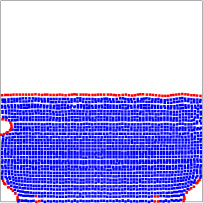
\includegraphics[width=0.7\textwidth]{13-1.png}
\caption{Particle distribution with basic Lagrangian FVPM (Red points are free surface).}\label{fig:13-1}
\end{minipage}
\begin{minipage}[t]{0.04\linewidth}
~
\end{minipage}
\begin{minipage}[t]{0.3\linewidth}
\centering
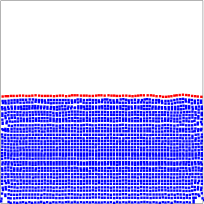
\includegraphics[width=0.7\textwidth]{13-2.png}
\caption{Particle distribution with Lagrangian particle motion and free surface detection (Red points are free surface).}\label{fig:13-2}
\end{minipage}
\begin{minipage}[t]{0.04\linewidth}
~
\end{minipage}
\begin{minipage}[t]{0.3\linewidth}
\centering
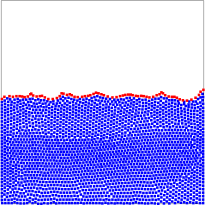
\includegraphics[width=0.7\textwidth]{13-3.png}
\caption{Particle distribution with particle transport correction and free surface detection (Red points are free surface).}\label{fig:13-3}
\end{minipage}
\end{figure}

The second test case is a translating rotating square in which the regions without particles are seen in Figures \ref{fig:13-4} to \ref{fig:13-9}. The voids can be treated if correct free-surface particle detection is implemented by the new method (Figures \ref{fig:13-10} to \ref{fig:13-12}).

\begin{figure}[!htb]
\begin{minipage}[t]{0.3\linewidth}
\centering
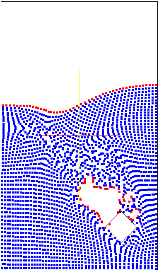
\includegraphics[width=0.6\textwidth]{13-4.png}
\caption{Particle distribution with basic Lagrangian FVPM, $t=0.52313$ s (Red points are free surface).}\label{fig:13-4}
\end{minipage}
\begin{minipage}[t]{0.04\linewidth}
~
\end{minipage}
\begin{minipage}[t]{0.3\linewidth}
\centering
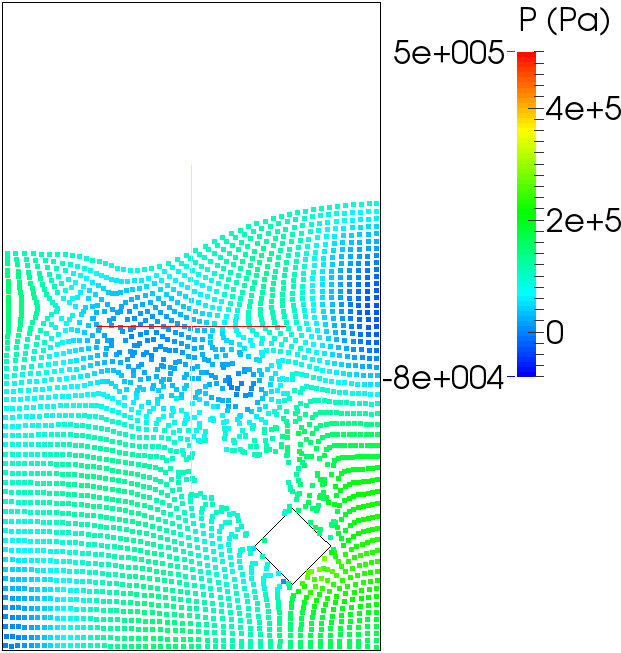
\includegraphics[width=0.975\textwidth]{13-5.png}
\caption{Pressure distribution with basic Lagrangian FVPM, $t=0.52313$ s.}\label{fig:13-5}
\end{minipage}
\begin{minipage}[t]{0.04\linewidth}
~
\end{minipage}
\begin{minipage}[t]{0.3\linewidth}
\centering
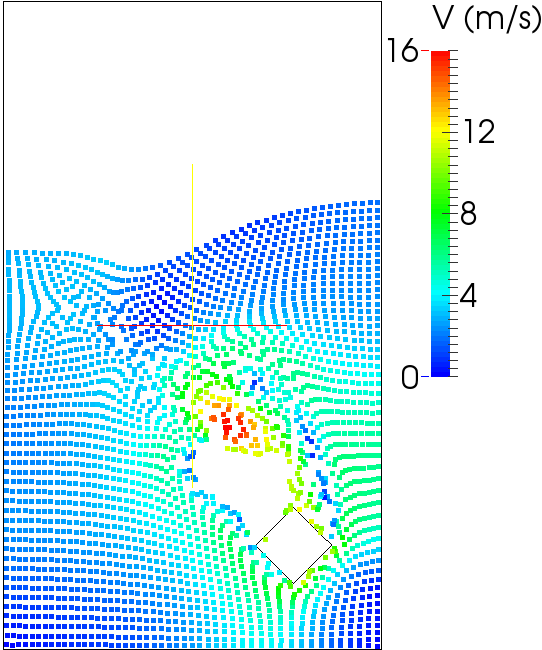
\includegraphics[width=0.865\textwidth]{13-6.png}
\caption{Velocity field with basic Lagrangian FVPM, $t=0.52313$ s.}\label{fig:13-6}
\end{minipage}\\
%-----------------------------------------
\begin{minipage}[t]{0.3\linewidth}
\centering
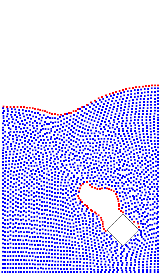
\includegraphics[width=0.6\textwidth]{13-7.png}
\caption{Particle distribution with particle transport correction, $t=0.52313$ s (Red points are free surface).}\label{fig:13-7}
\end{minipage}
\begin{minipage}[t]{0.04\linewidth}
~
\end{minipage}
\begin{minipage}[t]{0.3\linewidth}
\centering
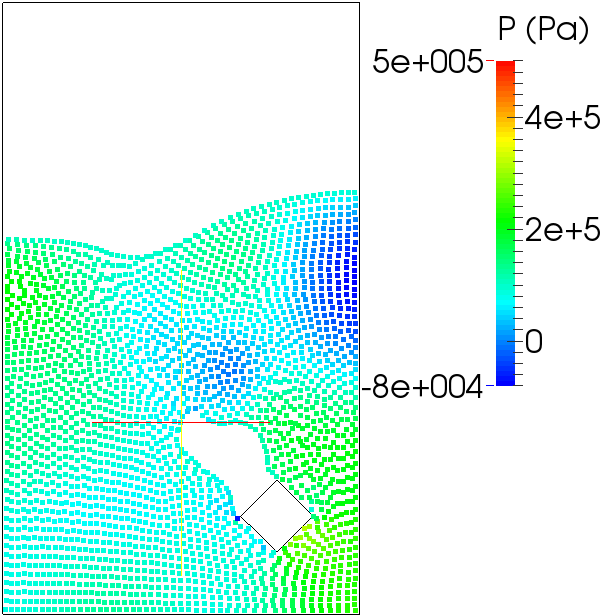
\includegraphics[width=0.975\textwidth]{13-8.png}
\caption{Pressure distribution with particle transport correction, $t=0.52313$ s.}\label{fig:13-8}
\end{minipage}
\begin{minipage}[t]{0.04\linewidth}
~
\end{minipage}
\begin{minipage}[t]{0.3\linewidth}
\centering
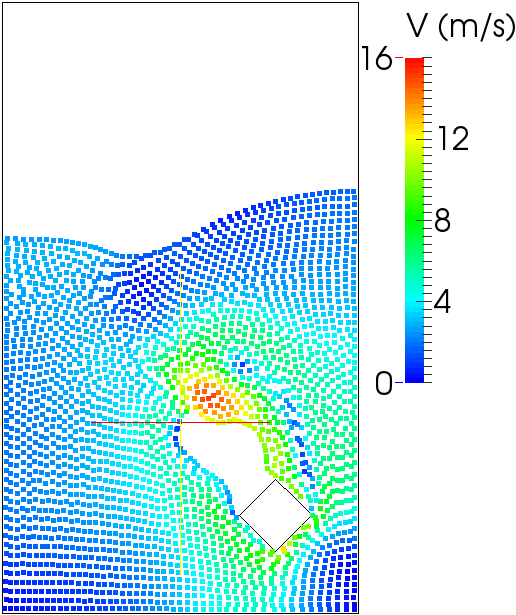
\includegraphics[width=0.865\textwidth]{13-9.png}
\caption{Velocity field with particle transport correction, $t=0.52313$ s.}\label{fig:13-9}
\end{minipage}\\
%-----------------------------------------
\begin{minipage}[t]{0.3\linewidth}
\centering
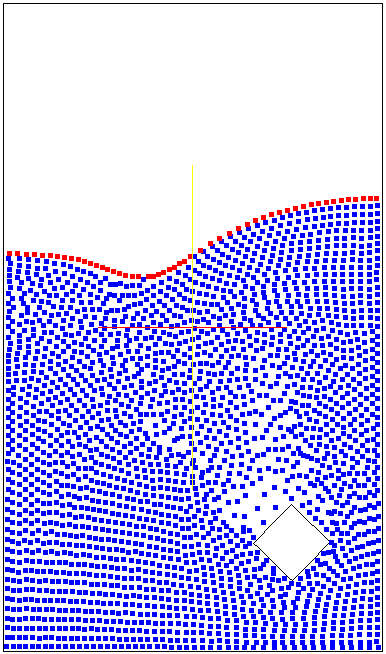
\includegraphics[width=0.6\textwidth]{13-10.png}
\caption{Particle distribution with particle transport correction and free surface detection, $t=0.52313$ s (Red points are free surface).}\label{fig:13-10}
\end{minipage}
\begin{minipage}[t]{0.04\linewidth}
~
\end{minipage}
\begin{minipage}[t]{0.3\linewidth}
\centering
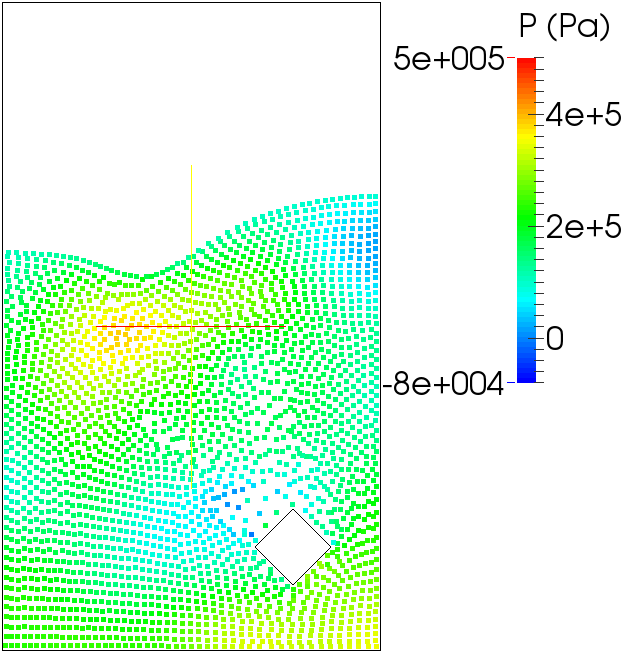
\includegraphics[width=0.975\textwidth]{13-11.png}
\caption{Pressure distribution with particle transport correction and free surface detection, $t=0.52313$ s.}\label{fig:13-11}
\end{minipage}
\begin{minipage}[t]{0.04\linewidth}
~
\end{minipage}
\begin{minipage}[t]{0.3\linewidth}
\centering
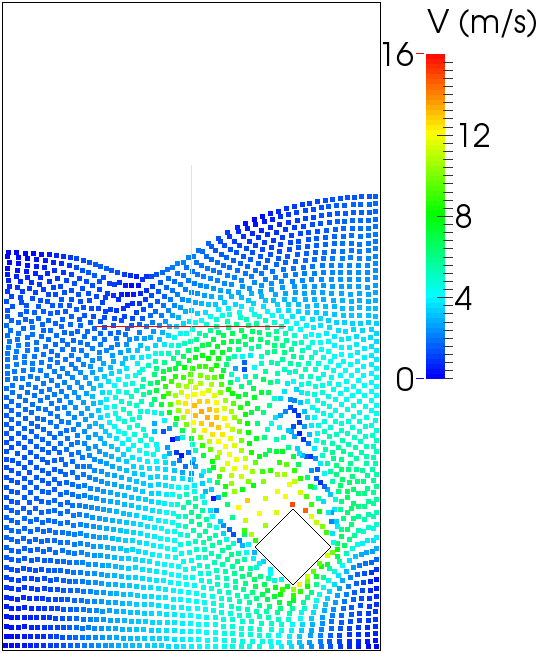
\includegraphics[width=0.865\textwidth]{13-12.png}
\caption{Velocity field with particle transport correction and free surface detection, $t=0.52313$ s.}\label{fig:13-12}
\end{minipage}
\end{figure}

\end{abstract}


%%THE END OF ABSTRACT

\addbib

\end{document}
